% 5-minute pitch: QOBLIB 08 network design, PushQuantum Hackathon 2026 (Qoro challenge).
% Build:  python3 make_numbers.py && latexmk -pdf pitch.tex
% make_numbers.py regenerates numbers.tex, results_table.tex and title_graph.tex from
% ../leaderboard/records.json, so re-run it right before the talk.
\documentclass[aspectratio=169,10pt]{beamer}
\usetheme[progressbar=frametitle,numbering=fraction,block=fill]{metropolis}
\usepackage[T1]{fontenc}
\usepackage[sfdefault,lining]{FiraSans}
\usepackage{booktabs}
\usepackage{array}
\usepackage{fontawesome5}
\usepackage{pifont}
\usepackage{tikz}
\usepackage{pgfplots}
\pgfplotsset{compat=1.18}
\usetikzlibrary{arrows.meta,calc,positioning,shapes.geometric,backgrounds}

% ---------------------------------------------------------------- colours
\definecolor{navy}{HTML}{0F172A}
\definecolor{ink}{HTML}{1E293B}
\definecolor{qblue}{HTML}{0369A1}
\definecolor{qcyan}{HTML}{38BDF8}
\definecolor{quantum}{HTML}{7C3AED}
\definecolor{good}{HTML}{059669}
\definecolor{bad}{HTML}{E11D48}
\definecolor{inc}{HTML}{EA8C00}
\definecolor{tie}{HTML}{64748B}
\definecolor{soft}{HTML}{EEF2F7}
\definecolor{muted}{HTML}{94A3B8}

\setbeamercolor{normal text}{fg=ink,bg=white}
\setbeamercolor{frametitle}{fg=white,bg=navy}
\setbeamercolor{progress bar}{fg=qcyan,bg=navy!80}
\setbeamercolor{title separator}{fg=qcyan}
\setbeamercolor{alerted text}{fg=bad}
\setbeamerfont{page number in head/foot}{size=\tiny}

\newcommand{\NumRecords}{12}
\newcommand{\NumRecordsQuantum}{12}
\newcommand{\NumTies}{3}
\newcommand{\NumInstances}{15}
\newcommand{\BestGap}{$-$3.4\,\%}
\newcommand{\BestGapN}{23}
\newcommand{\BigN}{24}
\newcommand{\BigVars}{552}
\newcommand{\BigBefore}{663\,688}
\newcommand{\BigAfter}{659\,539}
\newcommand{\BigGap}{$-$0.63\,\%}
\newcommand{\RecordsFrom}{network13}
\newcommand{\RecordsTo}{network24}
\newcommand{\Updated}{22 Nov 2026, 08:24}

\newcommand{\ResultsRows}{%
10 & 90 & 210\,800 & 210\,800 & \textcolor{tie}{$\pm$0.00\,\%} & \tikz[baseline=-0.6ex]\fill[tie] (0,0) circle (0.07); \\
11 & 110 & 238\,334 & 238\,334 & \textcolor{tie}{$\pm$0.00\,\%} & \tikz[baseline=-0.6ex]\fill[tie] (0,0) circle (0.07); \\
12 & 132 & 276\,474 & 276\,474 & \textcolor{tie}{$\pm$0.00\,\%} & \tikz[baseline=-0.6ex]\fill[tie] (0,0) circle (0.07); \\
13 & 156 & 300\,620 & \textbf{299\,715} & \textcolor{good}{\textbf{$-$0.30\,\%}} & \tikz[baseline=-0.6ex]\fill[good] (0,-0.09) rectangle (0.106,0.09); \\
14 & 182 & 343\,091 & \textbf{341\,375} & \textcolor{good}{\textbf{$-$0.50\,\%}} & \tikz[baseline=-0.6ex]\fill[good] (0,-0.09) rectangle (0.176,0.09); \\
15 & 210 & 370\,870 & \textbf{369\,720} & \textcolor{good}{\textbf{$-$0.31\,\%}} & \tikz[baseline=-0.6ex]\fill[good] (0,-0.09) rectangle (0.109,0.09); \\
16 & 240 & 397\,908 & \textbf{395\,566} & \textcolor{good}{\textbf{$-$0.59\,\%}} & \tikz[baseline=-0.6ex]\fill[good] (0,-0.09) rectangle (0.207,0.09); \\
17 & 272 & 437\,000 & \textbf{431\,938} & \textcolor{good}{\textbf{$-$1.16\,\%}} & \tikz[baseline=-0.6ex]\fill[good] (0,-0.09) rectangle (0.407,0.09); \\
18 & 306 & 473\,375 & \textbf{466\,000} & \textcolor{good}{\textbf{$-$1.56\,\%}} & \tikz[baseline=-0.6ex]\fill[good] (0,-0.09) rectangle (0.547,0.09); \\
19 & 342 & 492\,924 & \textbf{480\,000} & \textcolor{good}{\textbf{$-$2.62\,\%}} & \tikz[baseline=-0.6ex]\fill[good] (0,-0.09) rectangle (0.921,0.09); \\
20 & 380 & 528\,528 & \textbf{511\,769} & \textcolor{good}{\textbf{$-$3.17\,\%}} & \tikz[baseline=-0.6ex]\fill[good] (0,-0.09) rectangle (1.114,0.09); \\
21 & 420 & 569\,273 & \textbf{557\,053} & \textcolor{good}{\textbf{$-$2.15\,\%}} & \tikz[baseline=-0.6ex]\fill[good] (0,-0.09) rectangle (0.754,0.09); \\
22 & 462 & 618\,135 & \textbf{597\,524} & \textcolor{good}{\textbf{$-$3.33\,\%}} & \tikz[baseline=-0.6ex]\fill[good] (0,-0.09) rectangle (1.172,0.09); \\
23 & 506 & 659\,369 & \textbf{636\,848} & \textcolor{good}{\textbf{$-$3.42\,\%}} & \tikz[baseline=-0.6ex]\fill[good] (0,-0.09) rectangle (1.200,0.09); \\
24 & 552 & 663\,688 & \textbf{659\,539} & \textcolor{good}{\textbf{$-$0.63\,\%}} & \tikz[baseline=-0.6ex]\fill[good] (0,-0.09) rectangle (0.220,0.09); \\}


\newcommand{\goal}[1]{{\small\color{qblue}#1}\par\vspace{0.5em}}
\newcommand{\src}[1]{\par\vfill{\tiny\color{muted}#1}\par\vspace{-0.4em}}
\newcommand{\bignum}[2]{{\fontsize{22}{24}\selectfont\bfseries\color{#1}#2}}
\newcommand{\card}[2][0.95\linewidth]{%
  \tikz\node[fill=soft,rounded corners=3pt,inner sep=5pt,text width=#1,align=left]{#2};}

% ---------------------------------------------------------------- map of Germany
% Outline: Natural Earth via world.geo.json (public domain), equirectangular, x scaled by cos(51 deg).
\newcommand{\germany}{(-0.33,3.83) -- (-0.32,3.45) -- (0.31,3.21) -- (0.31,2.86) -- (0.94,3.05) -- (1.30,3.32) -- (2.01,2.93) -- (2.30,2.61) -- (2.45,2.10) -- (2.27,1.83) -- (2.50,1.47) -- (2.66,0.94) -- (2.61,0.60) -- (2.86,-0.04) -- (2.58,-0.15) -- (2.42,-0.03) -- (2.26,-0.22) -- (1.81,-0.42) -- (1.58,-0.67) -- (1.12,-0.88) -- (1.23,-1.18) -- (1.30,-1.60) -- (1.62,-1.84) -- (1.97,-2.27) -- (1.75,-2.73) -- (1.53,-2.86) -- (1.62,-3.51) -- (1.56,-3.68) -- (1.36,-3.48) -- (1.06,-3.45) -- (0.61,-3.63) -- (0.06,-3.58) -- (-0.03,-3.85) -- (-0.35,-3.57) -- (-0.54,-3.62) -- (-1.21,-3.32) -- (-1.34,-3.54) -- (-1.87,-3.53) -- (-1.79,-2.82) -- (-1.47,-2.13) -- (-2.38,-1.95) -- (-2.67,-1.69) -- (-2.64,-1.25) -- (-2.76,-1.02) -- (-2.69,-0.35) -- (-2.80,0.70) -- (-2.42,0.70) -- (-2.26,1.08) -- (-2.11,1.99) -- (-2.22,2.33) -- (-2.10,2.54) -- (-1.58,2.60) -- (-1.46,2.38) -- (-1.03,2.87) -- (-1.18,3.25) -- (-1.21,3.81) -- (-0.73,3.68) -- cycle}

\tikzset{
  city/.style={circle,fill=navy,draw=white,line width=0.9pt,minimum size=7.5pt,inner sep=0pt},
  clabel/.style={font=\scriptsize\bfseries,text=navy,fill=white,fill opacity=0.85,text opacity=1,
                 inner sep=1.2pt,rounded corners=1.5pt},
  road/.style={-{Stealth[length=2.3mm,width=1.9mm]},line width=1.1pt,draw=qblue,
               shorten >=3.8pt,shorten <=3.8pt},
  hot/.style={road,draw=bad,line width=1.8pt},
  faded/.style={road,draw=muted!45,line width=0.9pt},
  outroad/.style={road,draw=good,line width=2pt},
  inroad/.style={road,draw=inc,line width=2pt},
  titlearc/.style={draw=qcyan,opacity=0.5,line width=0.6pt},
  titlenode/.style={fill=qcyan},
}

% cities: 0 Berlin, 1 Munich, 2 Frankfurt, 3 Hamburg, 4 Cologne (QOBLIB network05 node order)
\newcommand{\cities}{%
  \node[city] (Ber) at (1.85,1.37) {};
  \node[city] (Mun) at (0.71,-3.01) {};
  \node[city] (Fra) at (-1.11,-1.04) {};
  \node[city] (Ham) at (-0.29,2.40) {};
  \node[city] (Col) at (-2.19,-0.21) {};
}
\newcommand{\citylabels}{%
  \node[clabel,right=3pt] at (Ber) {Berlin};
  \node[clabel,right=4pt] at (Mun) {Munich};
  \node[clabel,below=4pt] at (Fra) {Frankfurt};
  \node[clabel,above left=1pt and 0pt] at (Ham) {Hamburg};
  \node[clabel,above=4pt] at (Col) {Cologne};
}

% landscape for the warm-start slide
\pgfmathdeclarefunction{land}{1}{%
  \pgfmathparse{3.2+0.75*sin(1.7*#1 r)+0.45*sin((4.1*#1+0.6) r)-2.0*exp(-((#1-7.0)^2)/0.45)+0.03*(#1-5)^2}%
}

% ================================================================
\begin{document}

% ---------------------------------------------------------------- 1. title
{
\setbeamercolor{background canvas}{bg=navy}
\begin{frame}[plain]
  \begin{tikzpicture}[remember picture,overlay]
    \begin{scope}[shift={($(current page.east)+(-3.4,0.1)$)}]
      \coordinate (t0) at (90.00:2.7);
\coordinate (t1) at (75.00:2.7);
\coordinate (t2) at (60.00:2.7);
\coordinate (t3) at (45.00:2.7);
\coordinate (t4) at (30.00:2.7);
\coordinate (t5) at (15.00:2.7);
\coordinate (t6) at (0.00:2.7);
\coordinate (t7) at (-15.00:2.7);
\coordinate (t8) at (-30.00:2.7);
\coordinate (t9) at (-45.00:2.7);
\coordinate (t10) at (-60.00:2.7);
\coordinate (t11) at (-75.00:2.7);
\coordinate (t12) at (-90.00:2.7);
\coordinate (t13) at (-105.00:2.7);
\coordinate (t14) at (-120.00:2.7);
\coordinate (t15) at (-135.00:2.7);
\coordinate (t16) at (-150.00:2.7);
\coordinate (t17) at (-165.00:2.7);
\coordinate (t18) at (-180.00:2.7);
\coordinate (t19) at (-195.00:2.7);
\coordinate (t20) at (-210.00:2.7);
\coordinate (t21) at (-225.00:2.7);
\coordinate (t22) at (-240.00:2.7);
\coordinate (t23) at (-255.00:2.7);
\draw[titlearc] (t0) -- (t2);
\draw[titlearc] (t0) -- (t4);
\draw[titlearc] (t1) -- (t13);
\draw[titlearc] (t1) -- (t16);
\draw[titlearc] (t2) -- (t17);
\draw[titlearc] (t2) -- (t21);
\draw[titlearc] (t3) -- (t5);
\draw[titlearc] (t3) -- (t22);
\draw[titlearc] (t4) -- (t6);
\draw[titlearc] (t4) -- (t11);
\draw[titlearc] (t5) -- (t7);
\draw[titlearc] (t5) -- (t10);
\draw[titlearc] (t6) -- (t19);
\draw[titlearc] (t6) -- (t20);
\draw[titlearc] (t7) -- (t9);
\draw[titlearc] (t7) -- (t13);
\draw[titlearc] (t8) -- (t0);
\draw[titlearc] (t8) -- (t14);
\draw[titlearc] (t9) -- (t3);
\draw[titlearc] (t9) -- (t17);
\draw[titlearc] (t10) -- (t0);
\draw[titlearc] (t10) -- (t12);
\draw[titlearc] (t11) -- (t1);
\draw[titlearc] (t11) -- (t5);
\draw[titlearc] (t12) -- (t11);
\draw[titlearc] (t12) -- (t18);
\draw[titlearc] (t13) -- (t15);
\draw[titlearc] (t13) -- (t19);
\draw[titlearc] (t14) -- (t1);
\draw[titlearc] (t14) -- (t9);
\draw[titlearc] (t15) -- (t16);
\draw[titlearc] (t15) -- (t21);
\draw[titlearc] (t16) -- (t6);
\draw[titlearc] (t16) -- (t12);
\draw[titlearc] (t17) -- (t15);
\draw[titlearc] (t17) -- (t18);
\draw[titlearc] (t18) -- (t14);
\draw[titlearc] (t18) -- (t23);
\draw[titlearc] (t19) -- (t10);
\draw[titlearc] (t19) -- (t22);
\draw[titlearc] (t20) -- (t7);
\draw[titlearc] (t20) -- (t8);
\draw[titlearc] (t21) -- (t3);
\draw[titlearc] (t21) -- (t8);
\draw[titlearc] (t22) -- (t2);
\draw[titlearc] (t22) -- (t23);
\draw[titlearc] (t23) -- (t4);
\draw[titlearc] (t23) -- (t20);
\fill[titlenode] (t0) circle (0.075);
\fill[titlenode] (t1) circle (0.075);
\fill[titlenode] (t2) circle (0.075);
\fill[titlenode] (t3) circle (0.075);
\fill[titlenode] (t4) circle (0.075);
\fill[titlenode] (t5) circle (0.075);
\fill[titlenode] (t6) circle (0.075);
\fill[titlenode] (t7) circle (0.075);
\fill[titlenode] (t8) circle (0.075);
\fill[titlenode] (t9) circle (0.075);
\fill[titlenode] (t10) circle (0.075);
\fill[titlenode] (t11) circle (0.075);
\fill[titlenode] (t12) circle (0.075);
\fill[titlenode] (t13) circle (0.075);
\fill[titlenode] (t14) circle (0.075);
\fill[titlenode] (t15) circle (0.075);
\fill[titlenode] (t16) circle (0.075);
\fill[titlenode] (t17) circle (0.075);
\fill[titlenode] (t18) circle (0.075);
\fill[titlenode] (t19) circle (0.075);
\fill[titlenode] (t20) circle (0.075);
\fill[titlenode] (t21) circle (0.075);
\fill[titlenode] (t22) circle (0.075);
\fill[titlenode] (t23) circle (0.075);

    \end{scope}
    \fill[qcyan] ($(current page.west)+(0.9,2.15)$) rectangle +(1.6,0.07);
    \node[anchor=north west,text width=9.0cm,align=left,white,font=\raggedright]
      at ($(current page.west)+(0.85,1.95)$)
      {{\fontsize{30}{33}\selectfont\bfseries Start in the\\right valley}\\[0.7em]
       {\large\color{qcyan} Quantum warm starts + LLM-evolved search\\for network design (QOBLIB 08)}\\[1.8em]
       {\normalsize Team SharQ}\\[0.3em]
       {\small\color{white!70} PushQuantum Hackathon 2026 \textperiodcentered{} Qoro Quantum Challenge}};
    \node[anchor=south east,font=\tiny,text=white!50,align=right]
      at ($(current page.south east)+(-0.4,0.25)$)
      {Background: our record network for 24 cities\\(\BigAfter{}; QOBLIB best known \BigBefore)};
  \end{tikzpicture}
\end{frame}
}

% ---------------------------------------------------------------- 2. the problem
\begin{frame}{The problem: which roads should we build?}
  \goal{Goal: route every traveller so that the \textbf{busiest road} carries as little traffic as possible.}
  \begin{columns}[T,onlytextwidth]
    \begin{column}{0.40\textwidth}
      \centering
      \begin{tikzpicture}[scale=0.71]
        \fill[soft,draw=muted!70,line width=0.6pt] \germany;
        \cities
        % option A: ring of neighbours, both ways (busiest road 83.0)
        \only<2>{
          \draw[hot]  (Ber) to[bend left=13] (Mun);  \draw[road] (Mun) to[bend left=13] (Ber);
          \draw[road] (Mun) to[bend left=13] (Fra);  \draw[road] (Fra) to[bend left=13] (Mun);
          \draw[road] (Fra) to[bend left=13] (Col);  \draw[road] (Col) to[bend left=13] (Fra);
          \draw[hot]  (Ham) to[bend left=13] (Col);  \draw[road] (Col) to[bend left=13] (Ham);
          \draw[road] (Ham) to[bend left=13] (Ber);  \draw[road] (Ber) to[bend left=13] (Ham);
        }
        % option B (busiest road 74.0)
        \only<3>{
          \draw[road] (Ber) to[bend left=13] (Mun);  \draw[road] (Mun) to[bend left=13] (Ber);
          \draw[hot]  (Ham) to[bend left=13] (Col);  \draw[road] (Col) to[bend left=13] (Ham);
          \draw[hot]  (Ber) -- (Fra);  \draw[road] (Mun) -- (Fra);
          \draw[road] (Fra) -- (Ham);  \draw[hot]  (Fra) -- (Col);
          \draw[hot]  (Ham) -- (Ber);  \draw[road] (Col) to[bend right=18] (Mun);
        }
        % option C: the optimum of all 216 valid networks (65.5)
        \only<4>{
          \draw[road] (Ber) -- (Mun);  \draw[hot]  (Ber) -- (Fra);
          \draw[road] (Mun) -- (Fra);  \draw[hot]  (Mun) to[bend left=18] (Col);
          \draw[road] (Fra) -- (Ham);  \draw[hot]  (Fra) -- (Col);
          \draw[hot]  (Ham) -- (Ber);  \draw[hot]  (Ham) -- (Mun);
          \draw[road] (Col) -- (Ber);  \draw[road] (Col) -- (Ham);
        }
        % the rule, shown on Frankfurt
        \only<5>{
          \draw[faded] (Ber) -- (Mun);  \draw[faded] (Mun) to[bend left=18] (Col);
          \draw[faded] (Ham) -- (Ber);  \draw[faded] (Ham) -- (Mun);
          \draw[faded] (Col) -- (Ber);  \draw[faded] (Col) -- (Ham);
          \draw[inroad]  (Ber) -- (Fra);  \draw[inroad]  (Mun) -- (Fra);
          \draw[outroad] (Fra) -- (Ham);  \draw[outroad] (Fra) -- (Col);
          \node[city,minimum size=10pt,draw=navy,fill=white,line width=1.6pt] at (Fra) {};
        }
        \citylabels
      \end{tikzpicture}
    \end{column}
    \begin{column}{0.57\textwidth}
      \footnotesize
      \textbf{Travel demand}\enspace{\color{muted}row = from, column = to}\\[0.25em]
      \newcommand{\z}{\textcolor{muted!70}{0}}
      \newcommand{\x}{\textcolor{muted!70}{--}}
      \setlength{\tabcolsep}{6pt}
      \renewcommand{\arraystretch}{0.95}
      \begin{tabular}{@{}l*{5}{r}@{}}
        \toprule
        & Ber & Mun & Fra & Ham & Col \\
        \midrule
        Berlin    & \x & 24 & 43 & 23 & 21 \\
        Munich    & \z & \x & \z & \z & 21 \\
        Frankfurt & 16 & \z & \x & 20 & 44 \\
        Hamburg   & 42 & 20 & 18 & \x & 40 \\
        Cologne   & \z & \z & \z & 40 & \x \\
        \bottomrule
      \end{tabular}

      \vspace{0.8em}
      \uncover<2->{%
      \textbf{Three ways to build the roads}\enspace{\color{muted}load on the}\enspace{\color{bad}busiest road}\\[0.25em]
      \setlength{\tabcolsep}{4pt}
      \begin{tabular}{@{}l l r@{}}
        \alt<2>{\color{qblue}\bfseries}{} A & \alt<2>{\color{qblue}}{}Neighbours, both ways & \alt<2>{\color{bad}\bfseries}{}83.0 \\
        \uncover<3->{\alt<3>{\color{qblue}\bfseries}{} B} & \uncover<3->{\alt<3>{\color{qblue}}{}A smarter mix} & \uncover<3->{\alt<3>{\color{bad}\bfseries}{}74.0} \\
        \uncover<4->{\alt<4>{\color{qblue}\bfseries}{} C} & \uncover<4->{\alt<4>{\color{qblue}}{}Best of all 216 valid networks} & \uncover<4->{\textcolor{good}{\bfseries 65.5}\,\textcolor{good}{\faStar}} \\
      \end{tabular}}

      \vspace{0.8em}
      \uncover<5>{\card{\textbf{The rule:} every city has exactly
          \textcolor{good}{\textbf{2 roads out}} and \textcolor{inc}{\textbf{2 roads in}}.
          Traffic may split over several routes.}}
    \end{column}
  \end{columns}
  \src{Demand and scores: QOBLIB instance \texttt{network05} (5 nodes, proven optimum 65.5); every valid network scored with the official routing LP.}
\end{frame}

% ---------------------------------------------------------------- 3. why it is hard
\begin{frame}{Small map, astronomical search space}
  \begin{columns}[T,onlytextwidth]
    \begin{column}{0.57\textwidth}
      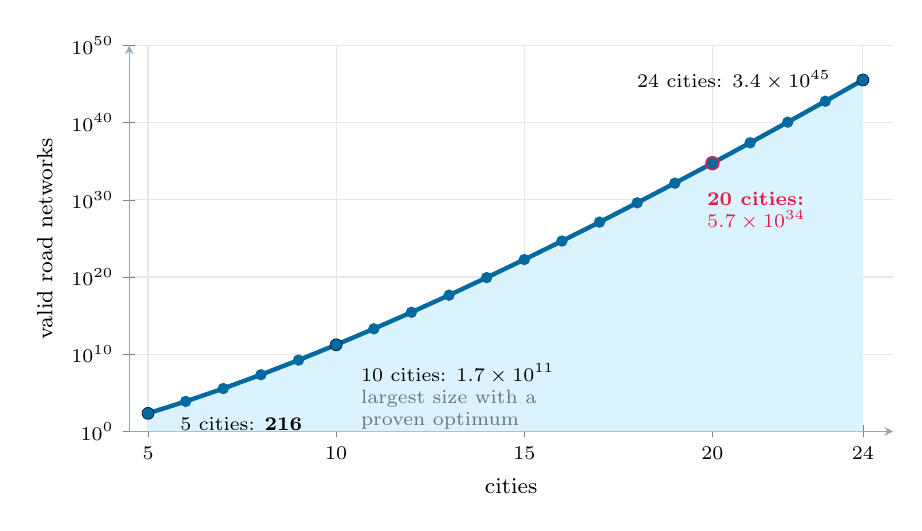
\begin{tikzpicture}
        \begin{axis}[
          scale only axis, width=0.80\linewidth, height=4.9cm,
          ymode=log, log basis y=10,
          xmin=4.5, xmax=24.8, ymin=1, ymax=1e50,
          xtick={5,10,15,20,24},
          ytick={1,1e10,1e20,1e30,1e40,1e50},
          xlabel={cities}, ylabel={valid road networks},
          tick label style={font=\scriptsize}, label style={font=\footnotesize},
          axis lines=left, axis line style={muted},
          grid=major, grid style={muted!25},
          clip=false,
        ]
          \addplot[draw=none,fill=qcyan!18] coordinates {(5,1) (5,2.1600e+02) (6,7.5700e+03) (7,3.5744e+05) (8,2.2040e+07) (9,1.7216e+09) (10,1.6626e+11) (11,1.9459e+13) (12,2.7148e+15) (13,4.4520e+17) (14,8.4798e+19) (15,1.8567e+22) (16,4.6314e+24) (17,1.3057e+27) (18,4.1315e+29) (19,1.4581e+32) (20,5.7068e+34) (21,2.4647e+37) (22,1.1692e+40) (23,6.0669e+42) (24,3.4301e+45) (24,1)} \closedcycle;
          \addplot[qblue,line width=1.6pt,mark=*,mark size=1.2pt] coordinates {(5,2.1600e+02) (6,7.5700e+03) (7,3.5744e+05) (8,2.2040e+07) (9,1.7216e+09) (10,1.6626e+11) (11,1.9459e+13) (12,2.7148e+15) (13,4.4520e+17) (14,8.4798e+19) (15,1.8567e+22) (16,4.6314e+24) (17,1.3057e+27) (18,4.1315e+29) (19,1.4581e+32) (20,5.7068e+34) (21,2.4647e+37) (22,1.1692e+40) (23,6.0669e+42) (24,3.4301e+45)};
          \fill[navy] (axis cs:5,216) circle (2.3pt);
          \node[font=\scriptsize,anchor=west,align=left] at (axis cs:5.6,10) {5 cities: \textbf{216}};
          \fill[navy] (axis cs:10,1.6626e11) circle (2.3pt);
          \node[font=\scriptsize,anchor=north west,align=left] at (axis cs:10.4,1e10) {10 cities: $1.7\times10^{11}$\\\textcolor{tie}{largest size with a}\\\textcolor{tie}{proven optimum}};
          \fill[bad] (axis cs:20,5.7068e34) circle (2.6pt);
          \node[font=\scriptsize,anchor=north west,align=left,text=bad] at (axis cs:19.6,2e32) {\textbf{20 cities:}\\\textbf{$5.7\times10^{34}$}};
          \fill[navy] (axis cs:24,3.4301e45) circle (2.3pt);
          \node[font=\scriptsize,anchor=east,align=right] at (axis cs:23.4,3e45) {24 cities: $3.4\times10^{45}$};
        \end{axis}
      \end{tikzpicture}
    \end{column}
    \begin{column}{0.40\textwidth}
      {\small Scoring one network (a routing LP):}\\[0.1em]
      \bignum{qblue}{$\approx$ 10 ms}\\[0.9em]
      {\small Trying every network for \textbf{20 cities}:}\\[0.1em]
      \bignum{bad}{$\approx 10^{25}$ years}\\[0.1em]
      {\footnotesize\color{tie} $10^{15}\times$ the age of the universe}\\[1.0em]
      {\small One yes/no variable per possible road:\\
       \textbf{552 binary variables} at 24 cities.}
    \end{column}
  \end{columns}
  \src{Exact counts of 2-in/2-out networks by dynamic programming (216 at 5 cities, confirmed by enumeration). LP time: official routing LP on network20.}
\end{frame}

% ---------------------------------------------------------------- 4. quantum warm start
\begin{frame}{Where you start decides where you end up}
  \begin{columns}[T,onlytextwidth]
    \begin{column}{0.56\textwidth}
      \begin{tikzpicture}[x=0.62cm,y=0.6cm]
        % terrain
        \fill[top color=qcyan!22,bottom color=white] plot[domain=0:11,samples=220,smooth] (\x,{land(\x)}) -- (11,-0.25) -- (0,-0.25) -- cycle;
        \draw[navy,line width=1.3pt] plot[domain=0:11,samples=220,smooth] (\x,{land(\x)});
        \draw[-{Stealth},muted,thick] (-0.3,-0.25) -- (-0.3,5.6);
        \node[font=\scriptsize,text=tie,rotate=90,anchor=south] at (-0.3,2.6) {busiest-road load};
        \node[font=\scriptsize,text=tie,anchor=north] at (5.5,-0.3) {all valid networks ($5.7\times10^{34}$ at 20 cities)};
        % best network
        \node[star,star points=5,star point ratio=2.2,fill=good,minimum size=9pt,inner sep=0pt] at (6.99,{land(6.99)}) {};
        \node[font=\scriptsize\bfseries,text=good,anchor=north] at (6.99,{land(6.99)-0.15}) {best network};
        % random starts get stuck
        \foreach \s/\e in {0.55/1.08, 3.15/2.60, 4.45/3.91, 5.30/5.86, 9.65/10.16} {
          \draw[-{Stealth[length=1.7mm]},muted,line width=0.9pt,yshift=7pt] plot[domain=\s:\e,samples=25,smooth] (\x,{land(\x)});
          \fill[muted] (\s,{land(\s)}) ++(0,3.2pt) circle (3.2pt);
          \draw[tie,line width=0.8pt] (\e,{land(\e)}) ++(-2.2pt,-2.2pt) -- ++(4.4pt,4.4pt) ++(-4.4pt,0) -- ++(4.4pt,-4.4pt);
        }
        \node[font=\scriptsize,text=tie,align=center,anchor=south] at (2.4,4.95) {random starts:\\stuck in shallow valleys};
        % quantum starts
        \uncover<2->{
          \foreach \s in {6.35,7.55,7.85} {
            \draw[-{Stealth[length=1.7mm]},quantum,line width=1.1pt,yshift=7pt] plot[domain=\s:6.99,samples=25,smooth] (\x,{land(\x)});
            \fill[quantum] (\s,{land(\s)}) ++(0,3.2pt) circle (3.2pt);
          }
          \node[font=\scriptsize\bfseries,text=quantum,align=center,anchor=south] at (8.7,4.6) {QAOA samples: start\\in the right valley};
        }
      \end{tikzpicture}
      \uncover<2->{%
      \footnotesize
      \textbf{Measured on network12}\enspace{\color{tie}gap to the best known value}\\[0.2em]
      \setlength{\tabcolsep}{5pt}
      \begin{tabular}{@{}lrr@{}}
        \toprule
        & best start & after 500 LP calls \\
        \midrule
        random starts & +18 to +24\,\% & +5.7\,\% \\
        \textcolor{quantum}{\textbf{QAOA starts}} & \textcolor{quantum}{\textbf{+9 to +17\,\%}} & \textcolor{quantum}{\textbf{+3.2\,\%}} \\
        \bottomrule
      \end{tabular}}
    \end{column}
    \begin{column}{0.41\textwidth}
      \uncover<2->{%
      \small
      \textbf{A quantum computer proposes the starting points}\\[0.4em]
      \footnotesize
      \card{{\color{quantum}\bfseries 1\enspace Encode.} One qubit per possible road. Roads that carry heavy demand get low energy; penalties enforce 2 in / 2 out.}\\[0.3em]
      \card{{\color{quantum}\bfseries 2\enspace Sample.} Partitioned QAOA with Qoro's Divi, blocks of 12--20 qubits, $p=2$, on the Qoro cloud.}\\[0.3em]
      \card{{\color{quantum}\bfseries 3\enspace Descend.} The lowest-energy samples give 100--200 starting networks; repair them, then search downhill with the routing LP.}}
    \end{column}
  \end{columns}
  \only<2->{\src{5 random start sets vs QAOA pools; the 500-call column uses the 2 QAOA pools held out from training. The head start narrows as the search budget grows.}}
\end{frame}

% ---------------------------------------------------------------- 5. ShinkaEvolve
\begin{frame}{An LLM evolves the algorithm: ShinkaEvolve}
  \begin{columns}[c,onlytextwidth]
    \begin{column}{0.50\textwidth}
      \centering
      \begin{tikzpicture}[
          box/.style={rounded corners=4pt,fill=soft,draw=qblue!60,line width=0.8pt,
                      text width=2.55cm,align=center,inner sep=4pt,font=\scriptsize},
          flow/.style={-{Stealth[length=2.4mm]},line width=1.3pt,qblue}]
        \node[box] (arch) at (0,2.05)  {{\color{qblue}\faDatabase}\enspace\textbf{Archive}\\islands of the best programs so far};
        \node[box] (llm)  at (2.25,0)  {{\color{qblue}\faRobot}\enspace\textbf{LLM edits code}\\proposes a diff to a parent program};
        \node[box] (run)  at (0,-2.05) {{\color{qblue}\faCogs}\enspace\textbf{Run on QOBLIB}\\QAOA samples $\rightarrow$ search $\rightarrow$ routing LP};
        \node[box] (score) at (-2.25,0) {{\color{qblue}\faChartLine}\enspace\textbf{Score}\\gap to best known, several instances and seeds};
        \draw[flow] (arch.east) to[bend left=30] (llm.north);
        \draw[flow] (llm.south) to[bend left=30] (run.east);
        \draw[flow] (run.west) to[bend left=30] (score.south);
        \draw[flow] (score.north) to[bend left=30] (arch.west);
        \node[font=\footnotesize\bfseries,text=navy,align=center] at (0,0) {{\large\faDna}\\[0.1em]evolution\\loop};
      \end{tikzpicture}
    \end{column}
    \begin{column}{0.47\textwidth}
      \small
      \textbf{We evolved two programs}\\[0.5em]
      \footnotesize
      \card{{\color{quantum}\bfseries\ding{172}\enspace The Hamiltonian}\enspace what the quantum circuit samples\\[0.3em]
            QAOA sample quality \textbf{0.74 $\rightarrow$ 0.84} {\color{tie}(1.0 = best known)}}\\[0.5em]
      \card{{\color{qblue}\bfseries\ding{173}\enspace The search}\enspace how to walk downhill from the quantum starts\\[0.3em]
            Gap on pools never seen in training \textbf{halved}: 3.5--5.0\,\% $\rightarrow$ \textbf{1.7--2.4\,\%}}\\[0.8em]
      {\color{tie}\faCheckCircle\enspace Winners re-tested on held-out pools and seeds\\[0.2em]
       \faCheckCircle\enspace Under \$4 of LLM calls per evolution run}
    \end{column}
  \end{columns}
  \src{Hamiltonian: partitioned QAOA on network12 (Maestro simulator), 4 seeds; quality = mean of (best known / best sample) and (best known / median sample). Search: network12, 2 held-out QAOA pools, 2000 LP calls, compared with our hand-written baseline search.}
\end{frame}

% ---------------------------------------------------------------- 6. results
\begin{frame}{Results: \NumRecords{} new best-known values on QOBLIB 08}
  \begin{columns}[T,onlytextwidth]
    \begin{column}{0.60\textwidth}
      \scriptsize
      \renewcommand{\arraystretch}{0.92}
      \setlength{\tabcolsep}{4.5pt}
      \begin{tabular}{@{}rrrrrl@{}}
        \toprule
        cities & variables & \textbf{before}: QOBLIB best & \textbf{ours} & gap & \\
        \midrule
        \ResultsRows
        \bottomrule
      \end{tabular}
    \end{column}
    \begin{column}{0.37\textwidth}
      \bignum{good}{\NumRecords\,/\,\NumInstances}\\[0.2em]
      {\footnotesize instances \textbf{below} QOBLIB's best known value; the other \NumTies{} tie it}\\[0.9em]
      \bignum{good}{\BestGap}\\[0.2em]
      {\footnotesize best improvement (\BestGapN{} cities)}\\[0.9em]
      {\footnotesize \textbf{Largest instance:} \BigN{} cities, \BigVars{} variables\\
       \BigBefore{} $\rightarrow$ \textbf{\BigAfter} (\BigGap)}\\[0.9em]
      {\footnotesize\color{quantum}\faAtom\enspace All \NumRecordsQuantum{} records start from QAOA samples.}
    \end{column}
  \end{columns}
  \src{Score = load on the busiest link $\times 1000$, lower is better. Every score recomputed by the official routing LP from our .sol files. Leaderboard as of \Updated.}
\end{frame}

% ---------------------------------------------------------------- 7. close
{
\setbeamercolor{background canvas}{bg=navy}
\begin{frame}[plain]
  \centering
  \vspace{1.2em}
  {\color{white}\fontsize{24}{28}\selectfont\bfseries Quantum picks the valley.\\[0.25em]
   Evolution learns the way down.}\\[1.4em]
  \begin{tikzpicture}[stat/.style={text width=3.6cm,align=center,font=\small,text=white}]
    \node[stat] (a) at (-4.3,0) {{\color{qcyan}\Large\faAtom}\\[0.3em]QAOA on Qoro\\proposes start networks};
    \node[stat] (b) at (0,0)    {{\color{qcyan}\Large\faDna}\\[0.3em]ShinkaEvolve writes\\the Hamiltonian and the search};
    \node[stat] (c) at (4.3,0)  {{\color{qcyan}\Large\faTrophy}\\[0.3em]\NumRecords{} new best-known\\values, up to \BigN{} cities};
  \end{tikzpicture}\\[1.8em]
  {\color{white}\Large Thank you!}\\[0.3em]
  {\small\color{white!65} Team SharQ \textperiodcentered{} PushQuantum Hackathon 2026}
\end{frame}
}

\end{document}
